% ------------------------------------------------------------------------------
% TYPO3 CMS 7.0 - What's New - Chapter "Backend User Interface" (German Version)
%
% @author	Patrick Lobacher <patrick@lobacher.de>
% @license	Creative Commons BY-NC-SA 3.0
% @link		http://typo3.org/download/release-notes/whats-new/
% @language	German
% ------------------------------------------------------------------------------
% LTXE-CHAPTER-UID:		e7264f0e-3f82290d-94c50cda-fb2d8e66
% LTXE-CHAPTER-NAME:	Backend User Interface
% ------------------------------------------------------------------------------

\section{Backend User Interface}
\begin{frame}[fragile]
	\frametitle{Backend User Interface}

	\begin{center}\huge{Kapitel 1:}\end{center}
	\begin{center}\huge{\color{typo3darkgrey}\textbf{Backend User Interface}}\end{center}

\end{frame}

% ------------------------------------------------------------------------------
% LTXE-SLIDE-START
% LTXE-SLIDE-UID:		68ceb369-26459388-130850ef-bd9c5af4
% LTXE-SLIDE-ORIGIN:	xxxxxxxx-xxxxxxxx-xxxxxxxx-xxxxxxxx
% LTXE-SLIDE-TITLE:		Allgemeines
% LTXE-SLIDE-REFERENCE:	https://forge.typo3.org/issues/62333
% LTXE-SLIDE-REFERENCE:	https://forge.typo3.org/issues/62995
% LTXE-SLIDE-REFERENCE:	https://forge.typo3.org/issues/62158
% LTXE-SLIDE-REFERENCE:	https://forge.typo3.org/issues/61454
% ------------------------------------------------------------------------------

\begin{frame}[fragile]
	\frametitle{Backend User Interface}
	\framesubtitle{Allgemeines}

	\begin{itemize}
		\item Das Backend User Interface wurde komplett überarbeitet
		\item Als Basis dient Twitter Bootstrap Version 3.2.x
		\item Sämtliche Icons wurden erneuert und grafisch im "Tile Style" überarbeitet
		\item Für Icons wird Font Awesome Version 4.2.x verwendet
		\item Linke Funktionenleiste wurde grafisch angepasst
		\item Icons wurden im Flat-Design, monochrom, farbig und mit abgerundeten Ecken entworfen
		\item Breite der Funktionenleiste kann soweit reduziert werden, dass nur noch Icos sichtbar sind
	\end{itemize}

\end{frame}


% ------------------------------------------------------------------------------
% LTXE-SLIDE-START
% LTXE-SLIDE-UID:		1c6a4d0e-b74c1295-010ffd20-7b90230c
% LTXE-SLIDE-ORIGIN:	xxxxxxxx-xxxxxxxx-xxxxxxxx-xxxxxxxx
% LTXE-SLIDE-TITLE:		Look & Feel (1)
% ------------------------------------------------------------------------------

\begin{frame}[fragile]
	\frametitle{Backend User Interface}
	\framesubtitle{Look \& Feel}

	\begin{figure}
		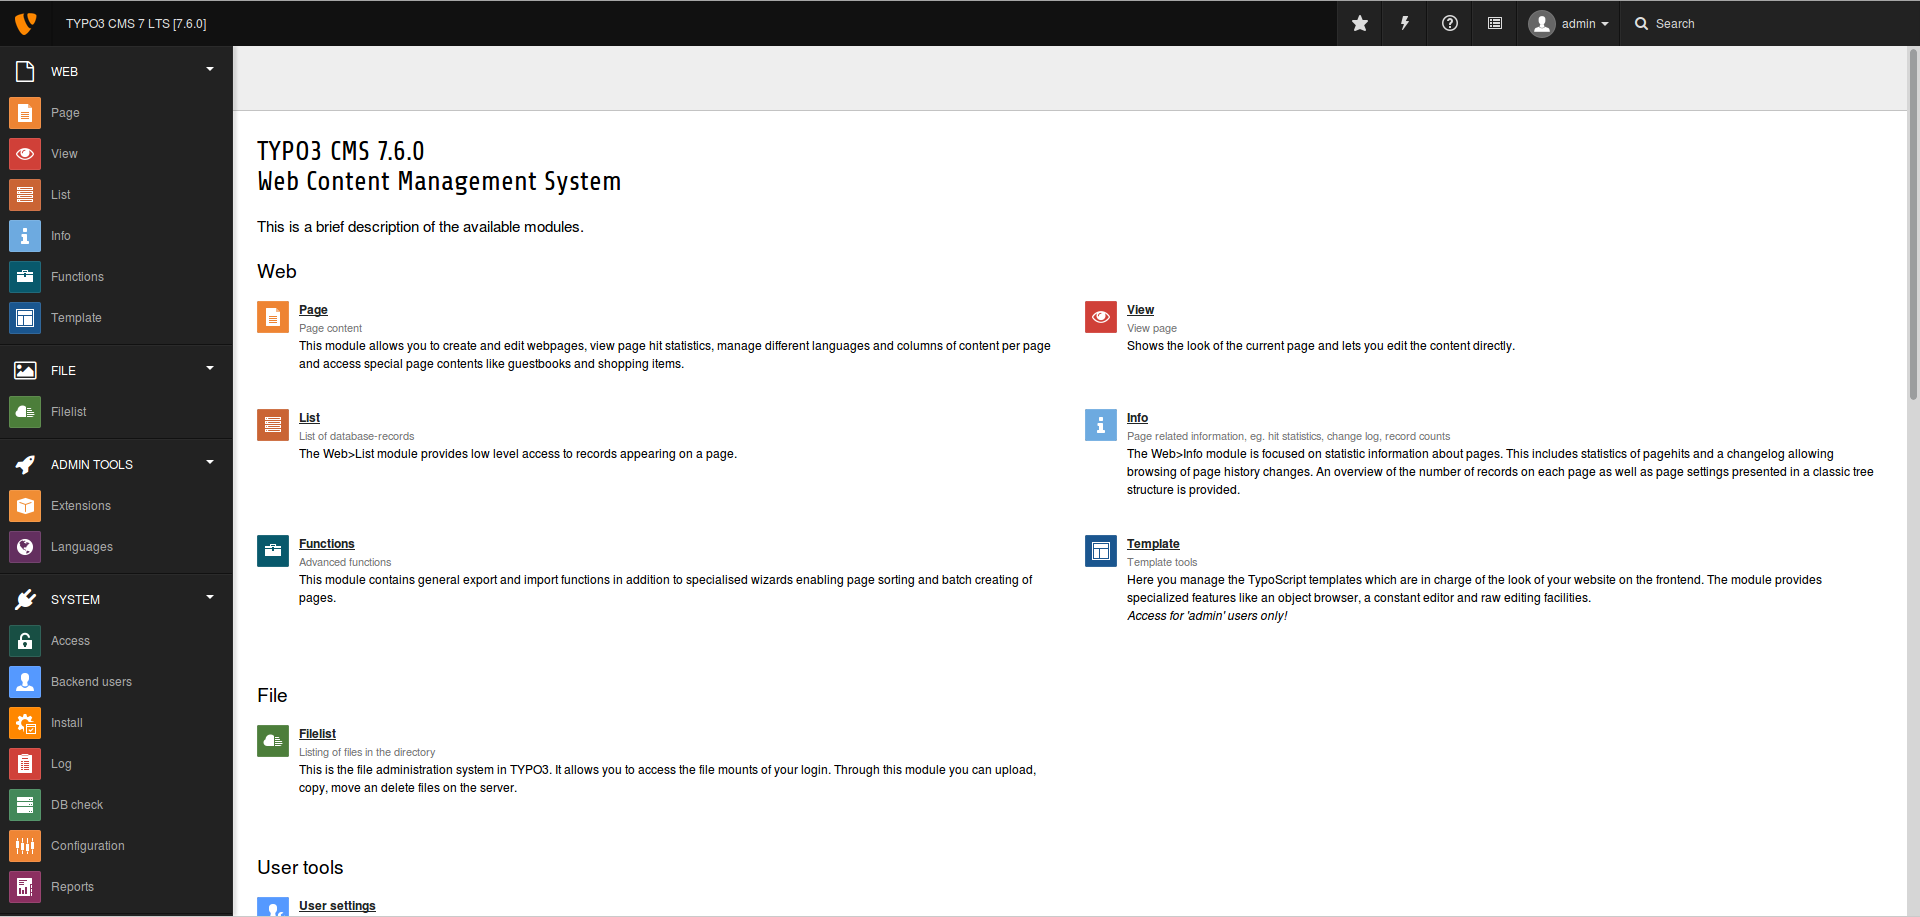
\includegraphics[width=0.90\linewidth]{BackendUserInterface/be-totalscreenshot1.png}
	\end{figure}

\end{frame}

% ------------------------------------------------------------------------------
% LTXE-SLIDE-START
% LTXE-SLIDE-UID:		b7755129-4a9e1437-1e26f21a-a9a87c1d
% LTXE-SLIDE-ORIGIN:	xxxxxxxx-xxxxxxxx-xxxxxxxx-xxxxxxxx
% LTXE-SLIDE-TITLE:		Look & Feel (2)
% ------------------------------------------------------------------------------

\begin{frame}[fragile]
	\frametitle{Backend User Interface}
	\framesubtitle{Look \& Feel}

	\begin{figure}
		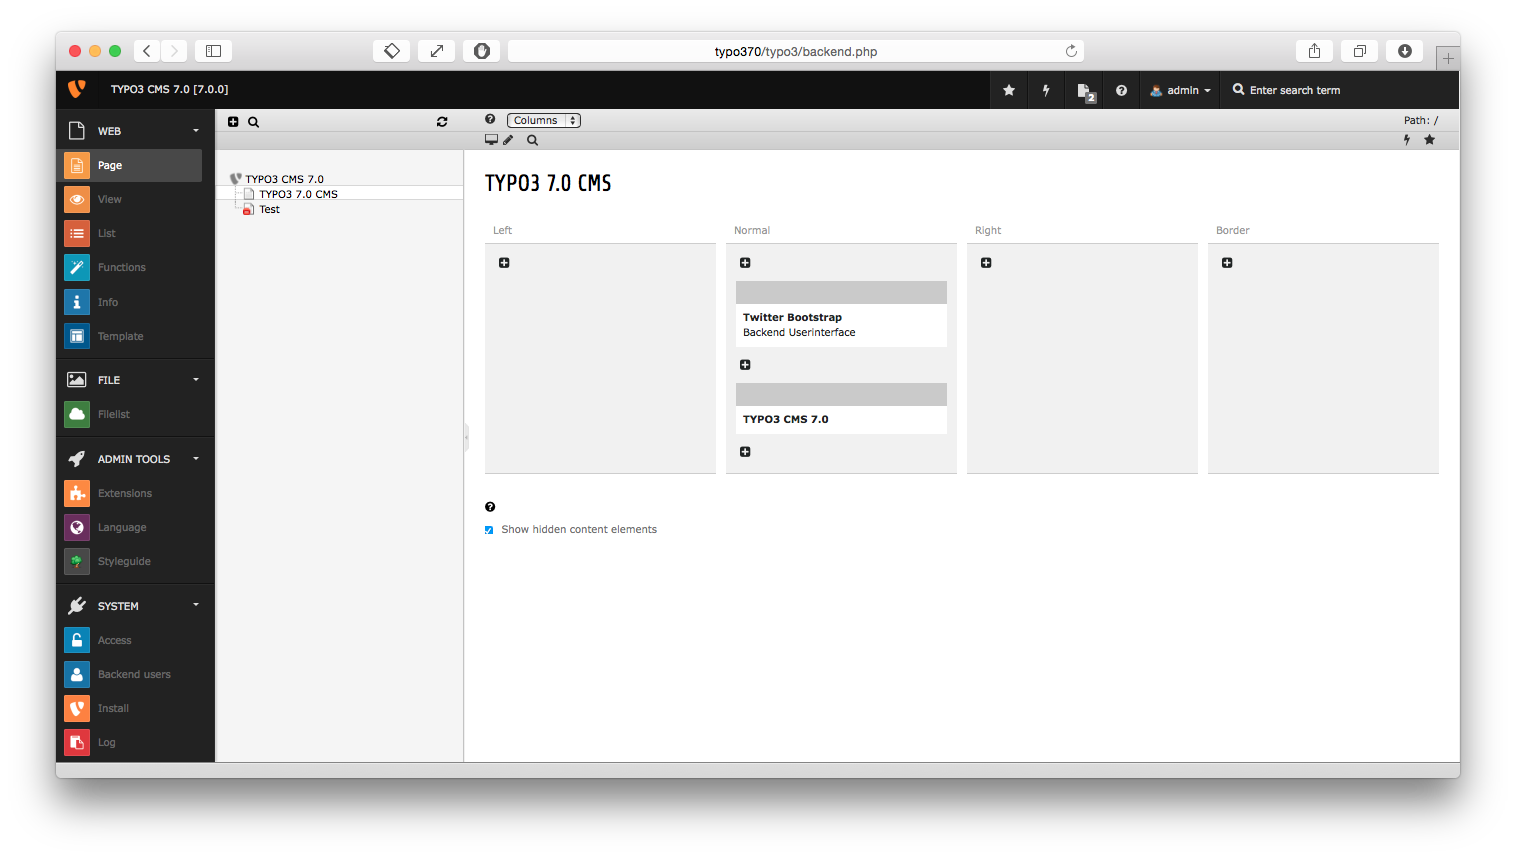
\includegraphics[width=0.90\linewidth]{BackendUserInterface/be-totalscreenshot2.png}
	\end{figure}

\end{frame}

% ------------------------------------------------------------------------------
% LTXE-SLIDE-START
% LTXE-SLIDE-UID:		a3222607-15908144-ab78ad9f-27d237c6
% LTXE-SLIDE-ORIGIN:	xxxxxxxx-xxxxxxxx-xxxxxxxx-xxxxxxxx
% LTXE-SLIDE-TITLE:		Look & Feel (3)
% ------------------------------------------------------------------------------

\begin{frame}[fragile]
	\frametitle{Backend User Interface}
	\framesubtitle{Look \& Feel}

	\begin{figure}
		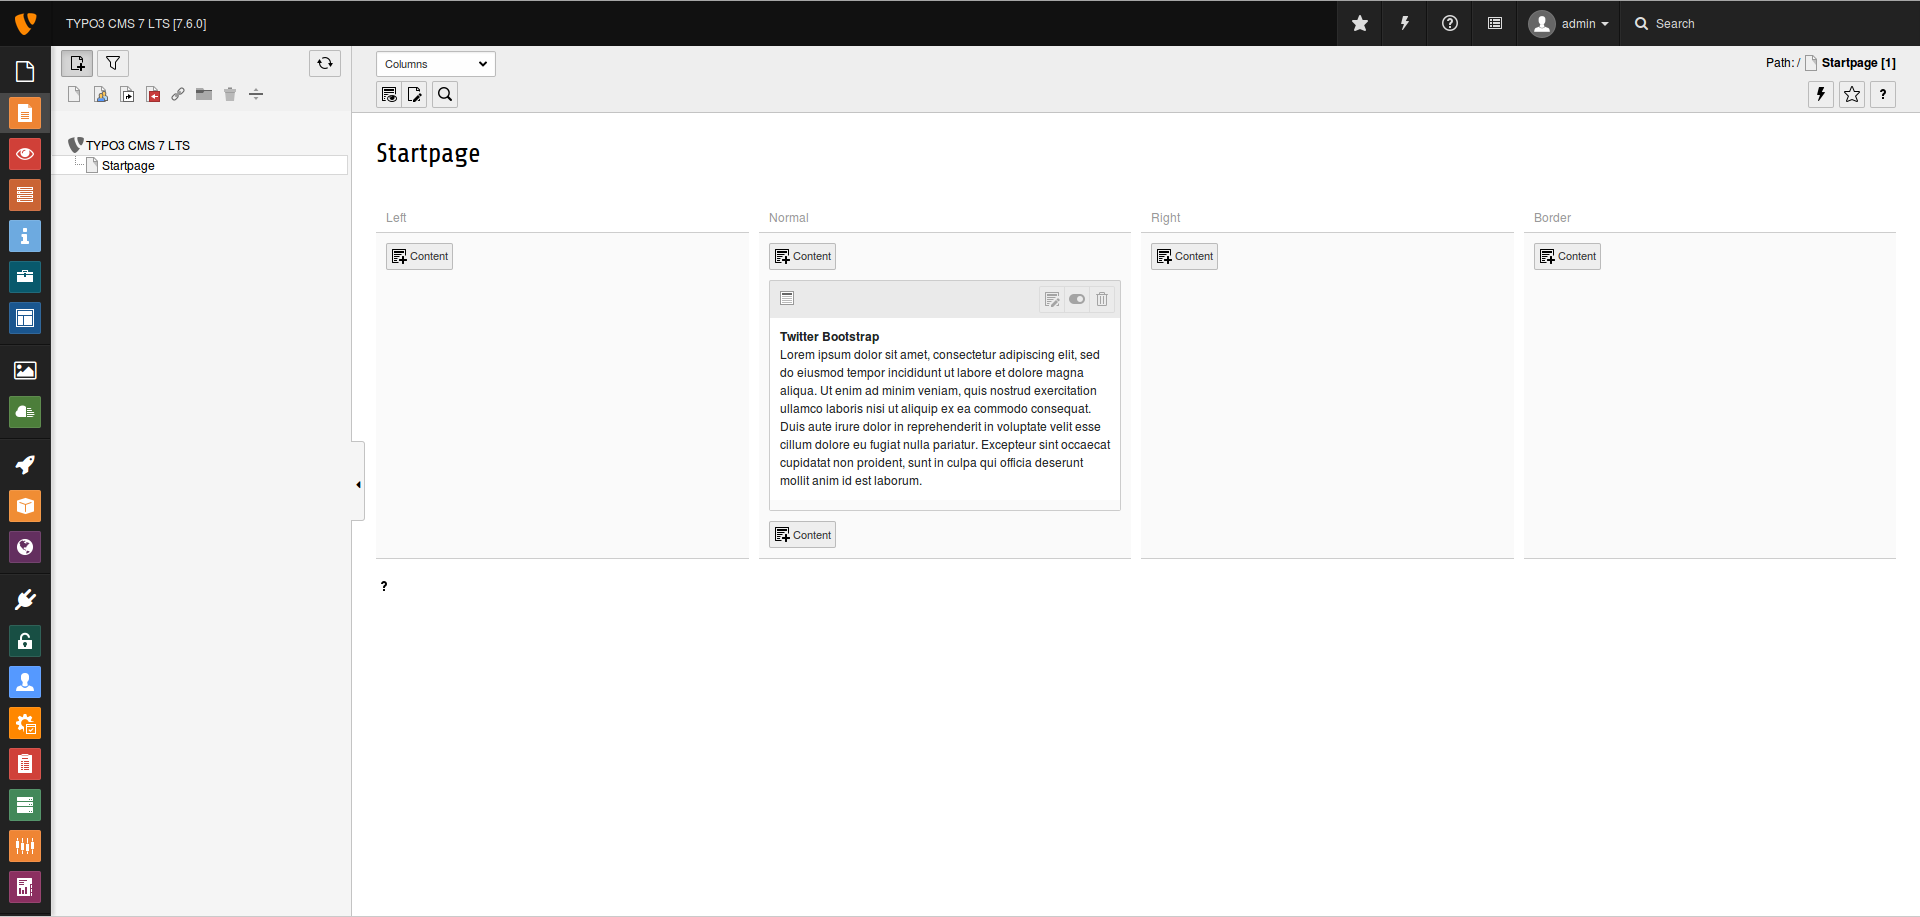
\includegraphics[width=0.90\linewidth]{BackendUserInterface/be-totalscreenshot3.png}
	\end{figure}

\end{frame}

% ------------------------------------------------------------------------------
% LTXE-SLIDE-START
% LTXE-SLIDE-UID:		08189c7f-c0772678-e797a207-51b42f9a
% LTXE-SLIDE-ORIGIN:	xxxxxxxx-xxxxxxxx-xxxxxxxx-xxxxxxxx
% LTXE-SLIDE-TITLE:		Backend User Login
% ------------------------------------------------------------------------------

\begin{frame}[fragile]
	\frametitle{Backend User Interface}
	\framesubtitle{Backend Benutzeranmeldung}

	\begin{figure}
		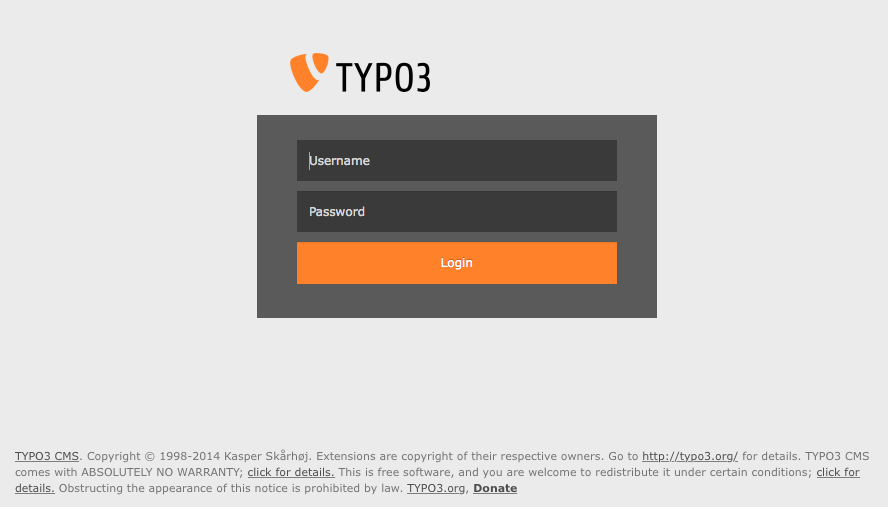
\includegraphics[width=0.80\linewidth]{BackendUserInterface/be-login.png}
	\end{figure}

\end{frame}

% ------------------------------------------------------------------------------
% LTXE-SLIDE-START
% LTXE-SLIDE-UID:		54542735-b3e97ff5-7b824e6b-97c8ade6
% LTXE-SLIDE-ORIGIN:	xxxxxxxx-xxxxxxxx-xxxxxxxx-xxxxxxxx
% LTXE-SLIDE-TITLE:		Refactor & recolor Modul Menu (Bootstrap)
% LTXE-SLIDE-REFERENCE:	https://forge.typo3.org/issues/62353
% ------------------------------------------------------------------------------

\begin{frame}[fragile]
	\frametitle{Backend User Interface}
	\framesubtitle{Top Bar (Module Menu)}

	\begin{figure}
		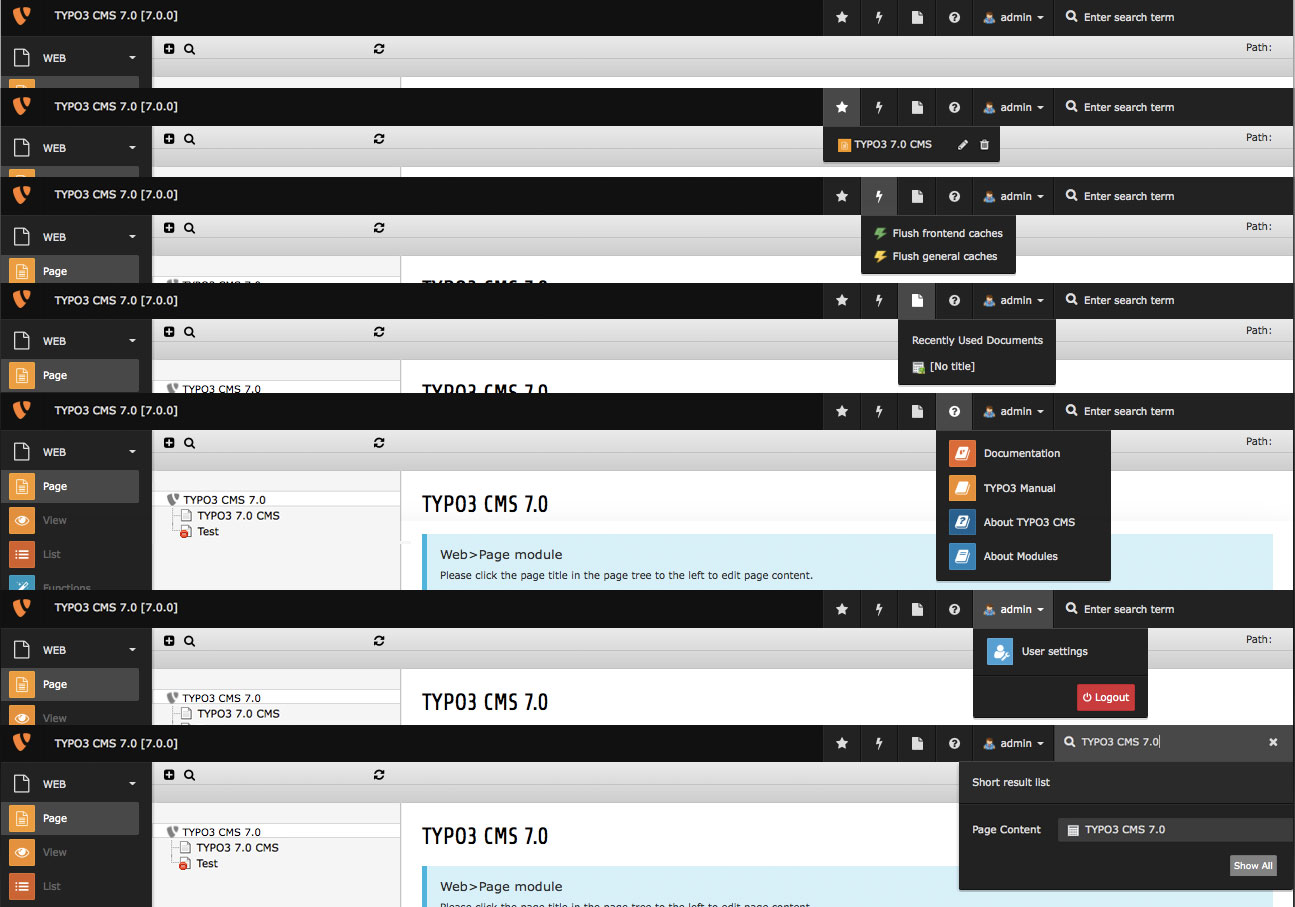
\includegraphics[width=0.70\linewidth]{BackendUserInterface/be-topbar.jpg}
	\end{figure}

\end{frame}

% ------------------------------------------------------------------------------
% LTXE-SLIDE-START
% LTXE-SLIDE-UID:		99b54aaf-067de9ac-8072e6dc-31b1e7a6
% LTXE-SLIDE-ORIGIN:	xxxxxxxx-xxxxxxxx-xxxxxxxx-xxxxxxxx
% LTXE-SLIDE-TITLE:		List Module und Clipboard
% LTXE-SLIDE-REFERENCE:	https://forge.typo3.org/issues/62963
% ------------------------------------------------------------------------------

\begin{frame}[fragile]
	\frametitle{Backend User Interface}
	\framesubtitle{Listen Modul und Zwischenablage}

	\begin{figure}
		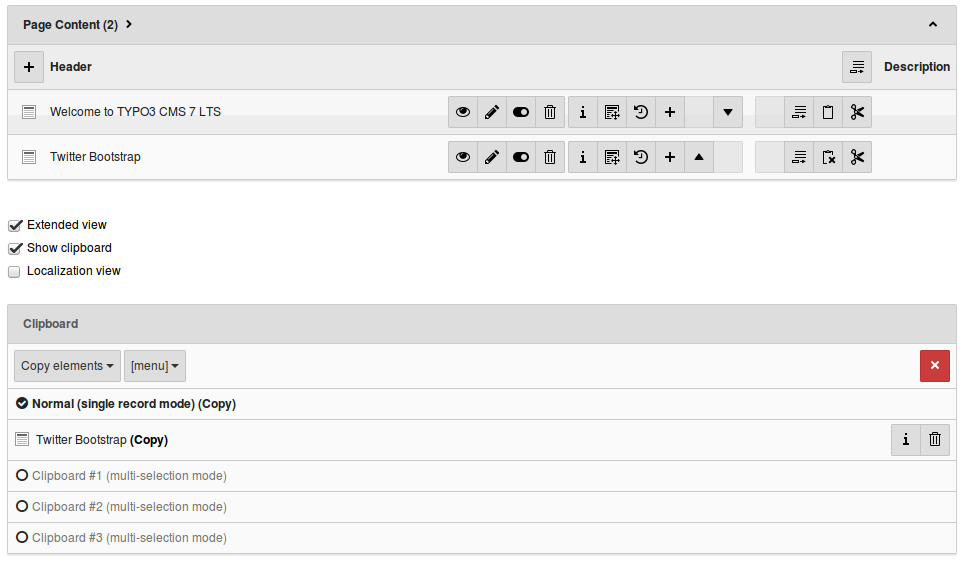
\includegraphics[width=0.80\linewidth]{BackendUserInterface/be-list.png}
	\end{figure}

\end{frame}

% ------------------------------------------------------------------------------
% LTXE-SLIDE-START
% LTXE-SLIDE-UID:		b1c6f367-889bce36-94a53be0-602ccdbc
% LTXE-SLIDE-ORIGIN:	xxxxxxxx-xxxxxxxx-xxxxxxxx-xxxxxxxx
% LTXE-SLIDE-TITLE:		Tabellenstil
% LTXE-SLIDE-REFERENCE:	https://forge.typo3.org/issues/62159
% ------------------------------------------------------------------------------

\begin{frame}[fragile]
	\frametitle{Backend User Interface}
	\framesubtitle{Tabellen}

	\begin{figure}
		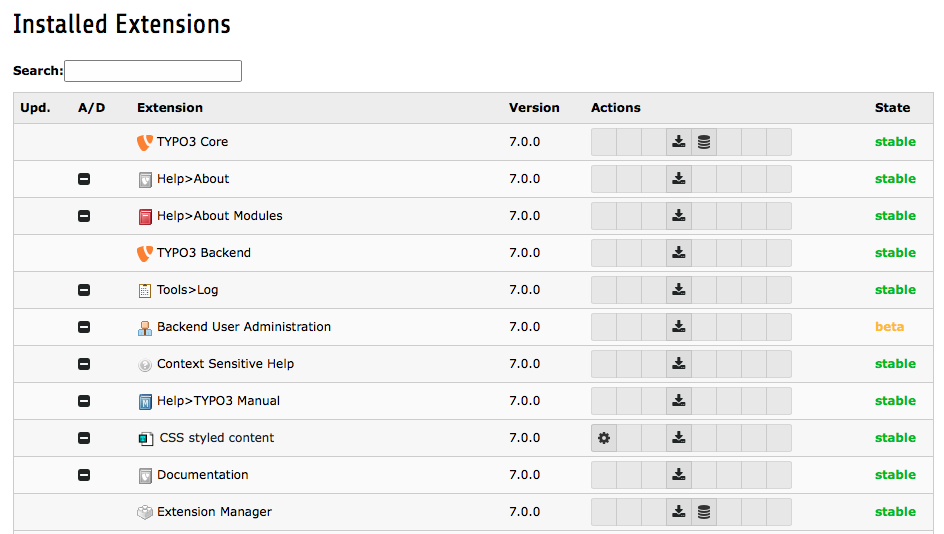
\includegraphics[width=0.99\linewidth]{BackendUserInterface/be-table.png}
	\end{figure}

\end{frame}

% ------------------------------------------------------------------------------
% LTXE-SLIDE-START
% LTXE-SLIDE-UID:		2be9330c-f6efda28-d7b8513c-7e14b424
% LTXE-SLIDE-ORIGIN:	xxxxxxxx-xxxxxxxx-xxxxxxxx-xxxxxxxx
% LTXE-SLIDE-TITLE:		Suche für Seite/Liste
% LTXE-SLIDE-REFERENCE:	https://forge.typo3.org/issues/59763
% ------------------------------------------------------------------------------

\begin{frame}[fragile]
	\frametitle{Backend User Interface}
	\framesubtitle{Suche für Seite/Liste}

	\begin{itemize}
		\item Klick auf die Lupe blendet eine Suche für die aktuelle Seite/Liste ein\newline
			(diese befand sich früher statisch am Ende der Seite)
	\end{itemize}

	\begin{figure}
		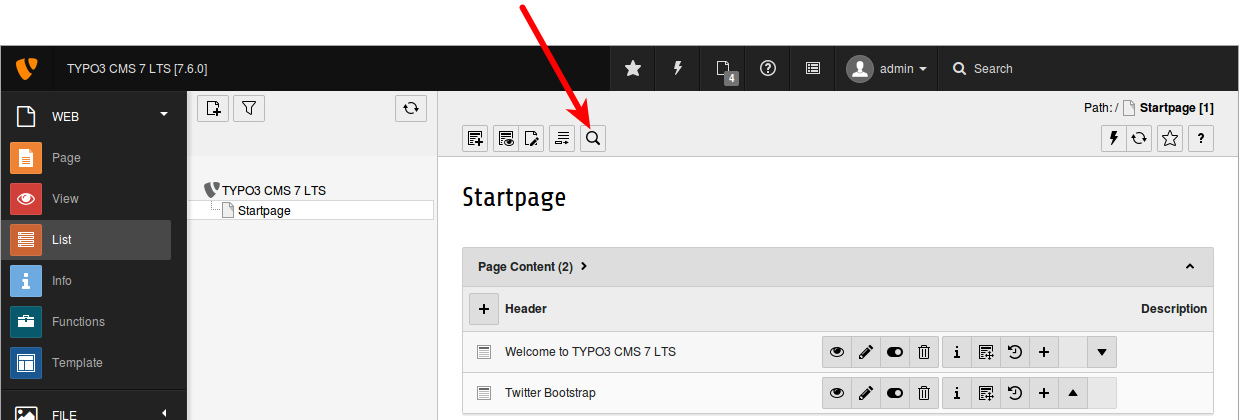
\includegraphics[width=0.95\linewidth]{BackendUserInterface/be-search.jpg}
	\end{figure}

\end{frame}

% ------------------------------------------------------------------------------
% LTXE-SLIDE-START
% LTXE-SLIDE-UID:		da4ad2d4-cd2c2f95-8adcbf62-4a5287f7
% LTXE-SLIDE-ORIGIN:	xxxxxxxx-xxxxxxxx-xxxxxxxx-xxxxxxxx
% LTXE-SLIDE-TITLE:		Anzahl offene Dokumente (Badge)
% LTXE-SLIDE-REFERENCE:	https://forge.typo3.org/issues/61675
% ------------------------------------------------------------------------------

\begin{frame}[fragile]
	\frametitle{Backend User Interface}
	\framesubtitle{Anzahl offene Dokumente}

	\begin{itemize}
		\item Anzahl offene Dokumente wird über ein Bootstrap "Badge" angezeigt\newline
			(setzt die installierte Extension "Open Documents" voraus)
	\end{itemize}
	\begin{figure}
		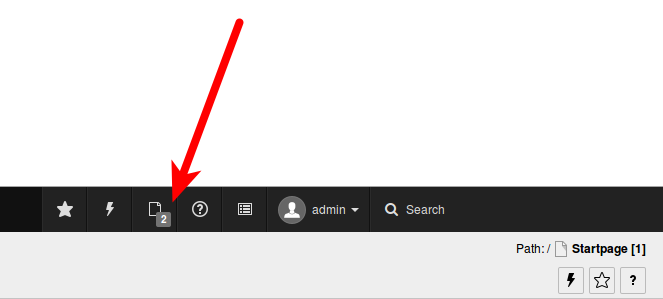
\includegraphics[width=0.75\linewidth]{BackendUserInterface/be-badge.png}
	\end{figure}

\end{frame}

% ------------------------------------------------------------------------------
% LTXE-SLIDE-START
% LTXE-SLIDE-UID:		1bfb82ab-000dd252-b2136f2b-d23bc787
% LTXE-SLIDE-ORIGIN:	xxxxxxxx-xxxxxxxx-xxxxxxxx-xxxxxxxx
% LTXE-SLIDE-TITLE:		FlashMessages
% LTXE-SLIDE-REFERENCE:	https://forge.typo3.org/issues/62580
% ------------------------------------------------------------------------------

\begin{frame}[fragile]
	\frametitle{Backend User Interface}
	\framesubtitle{Flash Messages}

	\begin{itemize}
		\item FlashMessage-Boxen im Backend wurden überarbeitet
		\item Dafür wurde der Kontrast von Text und Box erhöht und Links werden besser hervorgehoben
	\end{itemize}

	\begin{columns}[T]
		\begin{column}{.25\textwidth}
			\smaller\hfill 
				\begingroup\color{typo3red}TYPO3 CMS < 7.0\endgroup
			\normalsize
		\end{column}

		\begin{column}{.5\textwidth}
			\begin{figure}\vspace*{-0.6cm}
				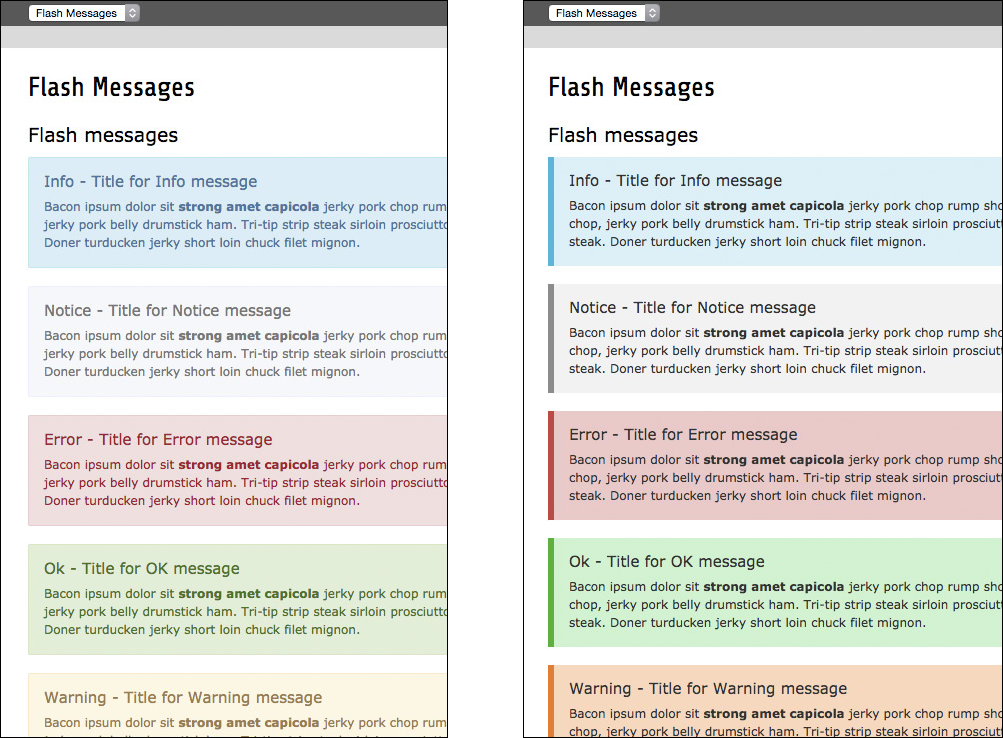
\includegraphics[width=0.99\linewidth]{BackendUserInterface/be-flashmessages.png}
			\end{figure}
		\end{column}

		\begin{column}{.25\textwidth}
			\smaller
				\begingroup\color{typo3red}TYPO3 CMS >= 7.0\endgroup
			\normalsize
		\end{column}
	\end{columns}

\end{frame}

% ------------------------------------------------------------------------------
% LTXE-SLIDE-START
% LTXE-SLIDE-UID:		6590a32a-3a0d0ec5-11f1297f-9f37e43d
% LTXE-SLIDE-ORIGIN:	xxxxxxxx-xxxxxxxx-xxxxxxxx-xxxxxxxx
% LTXE-SLIDE-TITLE:		Video Player in Info Window
% LTXE-SLIDE-REFERENCE:	https://forge.typo3.org/issues/61668
% ------------------------------------------------------------------------------

\begin{frame}[fragile]
	\frametitle{Backend User Interface}
	\framesubtitle{Video Player in Info Window}

	\begin{itemize}
		\item Ein Videoplayer ermöglicht es, HTML5 Audio- und Video-Dateien im "Info"-Fenster abzuspielen

		\begin{figure}
			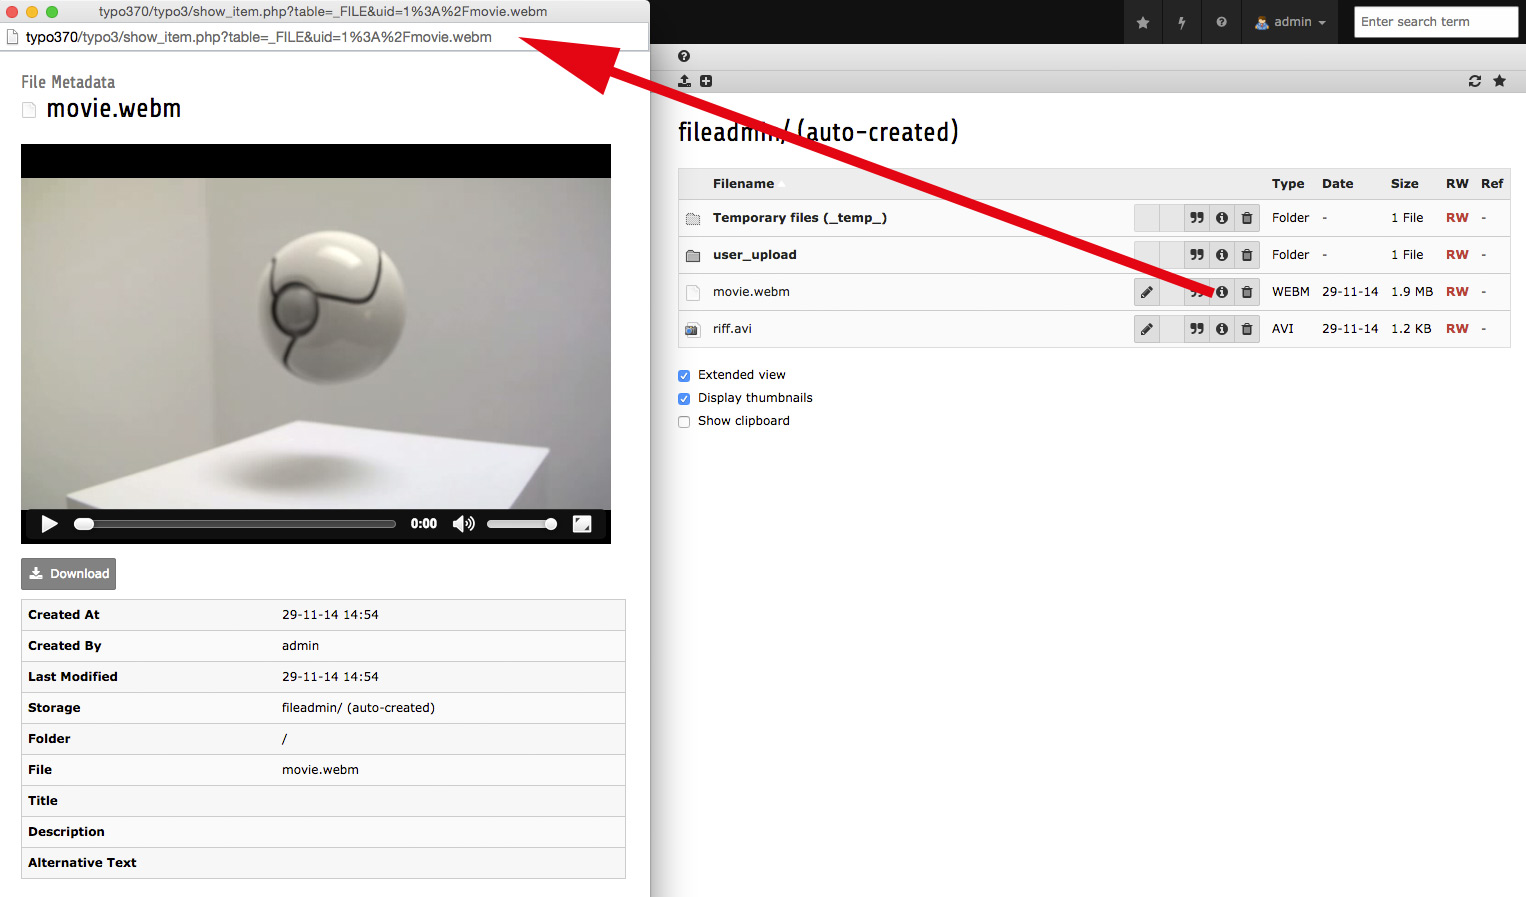
\includegraphics[width=0.70\linewidth]{BackendUserInterface/be-info.jpg}
		\end{figure}

	\end{itemize}

\end{frame}

% ------------------------------------------------------------------------------
